\begin{frame}
    \frametitle{Least Squares en General}
    \note{Extraído de Curso de Cyrill Stachniss https://youtu.be/r2cyMQ5NB1o?si=WYODHSkWun3FL7jR}
    
    Enfoque para calcular una solución para un sistema sobredeterminado

    \begin{itemize}
        \item Más ecuaciones que incógnitas
        \item Minimiza la suma de cuadrados de los errores en las ecuaciones
        \item Enfoque estándar para un gran conjunto de problemas
        \item Se utiliza para estimar el modelo de parámetros dado un conjunto de observaciones
    \end{itemize}
\end{frame}

\begin{frame}
    \frametitle{Nuestro Problema}
    \note{Extraído de Curso de Cyrill Stachniss https://youtu.be/r2cyMQ5NB1o?si=WYODHSkWun3FL7jR}
    
    Dado un sistema descripto por un conjunto de $n$ funciones de observación $\left\{f_{i}\left(\state\right)\right\}_{i=1:n}$

    \begin{itemize}
        \item $\stateBold$ es el vector de estado
        \item $\observationBold$ es una una medición del estado $\stateBold$
        \item $\prediction_{i} = f_{i}\left(\stateBold\right)$ es una función que mapea el estado $\stateBold$ a una medición predicha $\prediction_{i}$
        \item Dadas $n$ mediciones ruidosas $\observationBold_{1:n}$ acerca del estado $\stateBold$
        \item Objetivo: Estimar el estado $\stateBold$ que mejor explica las mediciones $\observationBold_{1:n}$
    \end{itemize}
\end{frame}

\begin{frame}
    \frametitle{Explicación Gráfica}
    \note{Extraído de Curso de Cyrill Stachniss https://youtu.be/r2cyMQ5NB1o?si=WYODHSkWun3FL7jR}
    
    \begin{center}
        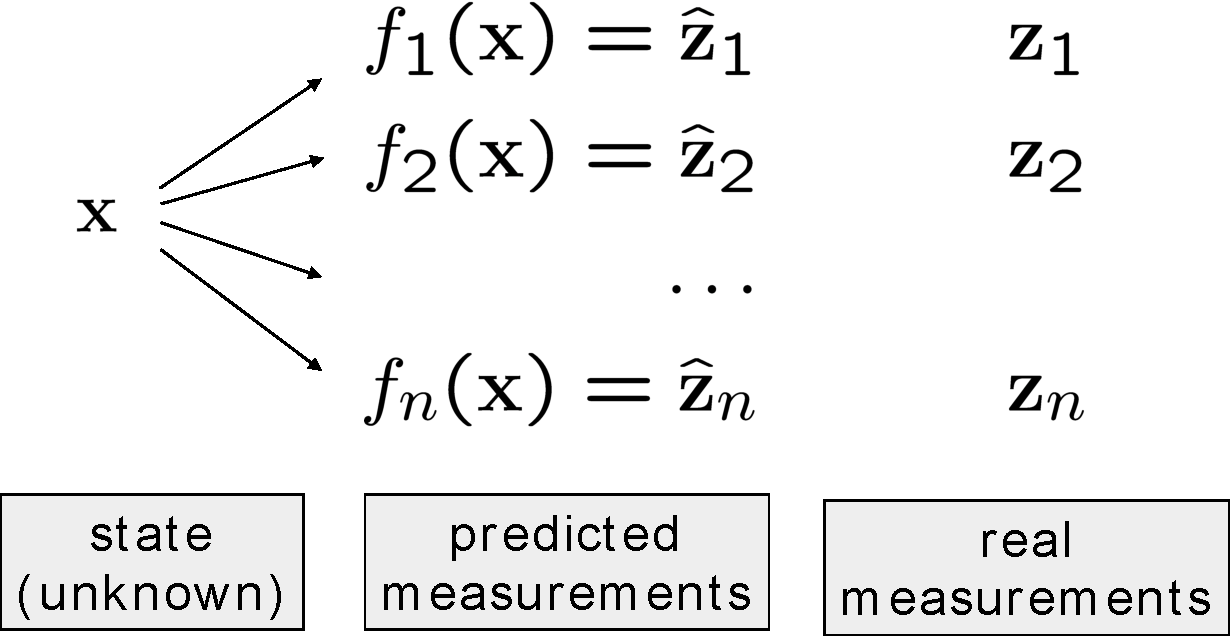
\includegraphics[width=0.7\textwidth]{images/least_squares.pdf}
    \end{center}

\end{frame}

\begin{frame}
    \frametitle{Ejemplo}
    \note{Extraído de Curso de Cyrill Stachniss https://youtu.be/r2cyMQ5NB1o?si=WYODHSkWun3FL7jR}
    
    \begin{center}
        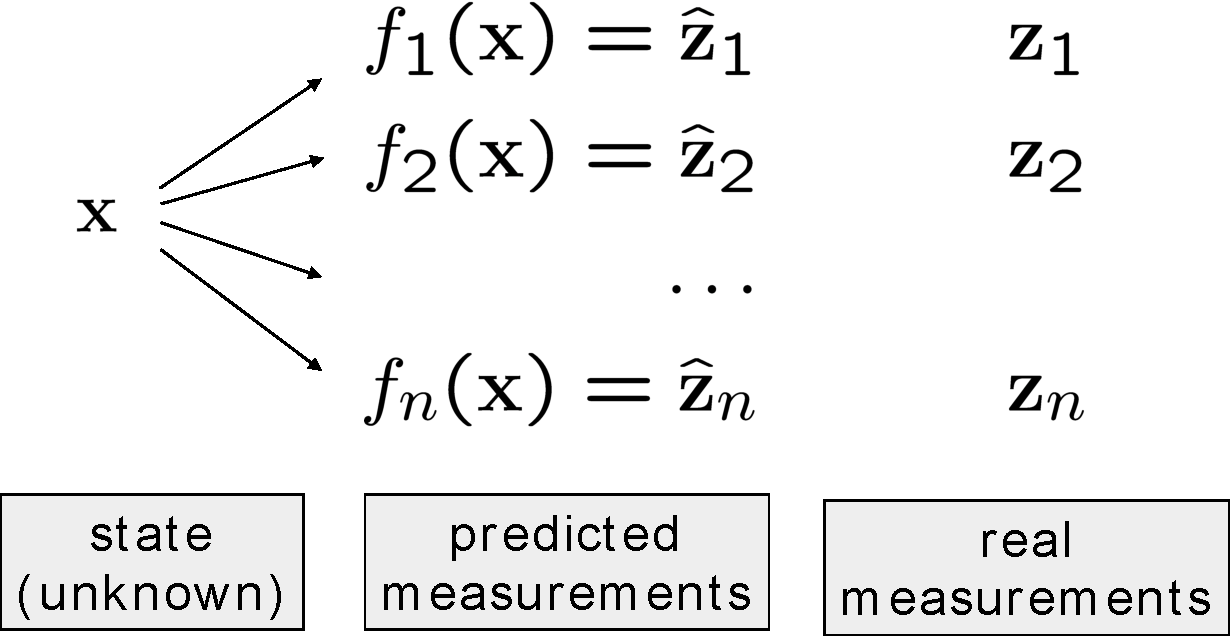
\includegraphics[width=0.7\textwidth]{images/least_squares.pdf}
    \end{center}
    
    \begin{itemize}
        \item $\stateBold$ posición de los puntos 3D
        \item $\observationBold_{i}$ coordenadas de los puntos 3D proyectados en las imágenes
        \item Estimar la posición 3D más probable de los puntos basado en las proyecciones en las imágenes (dada las poses de la cámara)
    \end{itemize}
\end{frame}

\begin{frame}
    \frametitle{Función de Error}
    \note{Extraído de Curso de Cyrill Stachniss https://youtu.be/r2cyMQ5NB1o?si=WYODHSkWun3FL7jR}
    
    \begin{itemize}
        \item El error $\error_{i}$ suele ser la diferencia entre la medición real y la predicción:
            \begin{equation*}
                \error_{i}\left( \stateBold \right) = \observationBold_{i} - f_{i}\left( \stateBold \right)
            \end{equation*}
        \item Supongamos que el error tiene una distribución normal con media cero y matriz covarianza $\covariance$
        \item La matriz de información del Error Gaussiano es $\informationMatrix_{i} = \inverse{\covariance}$
        \item El error al cuadrado de una medición depende sólo del estado y es un escalar:
            \begin{equation*}
                \error_{i}\left( \stateBold \right) = \error_{i}\left( \stateBold \right)^{\top} \informationMatrix_{i} \error_{i}\left( \stateBold \right)
            \end{equation*}
    \end{itemize}
\end{frame}

\begin{frame}
    \frametitle{Objetivo: Encontrar el Mínimo}
    \note{Extraído de Curso de Cyrill Stachniss https://youtu.be/r2cyMQ5NB1o?si=WYODHSkWun3FL7jR}
    
    \begin{itemize}
        \item Encontrar el estado $\stateBold^{*}$ que minimiza el error dados todas las mediciones
        
        \begin{center}
            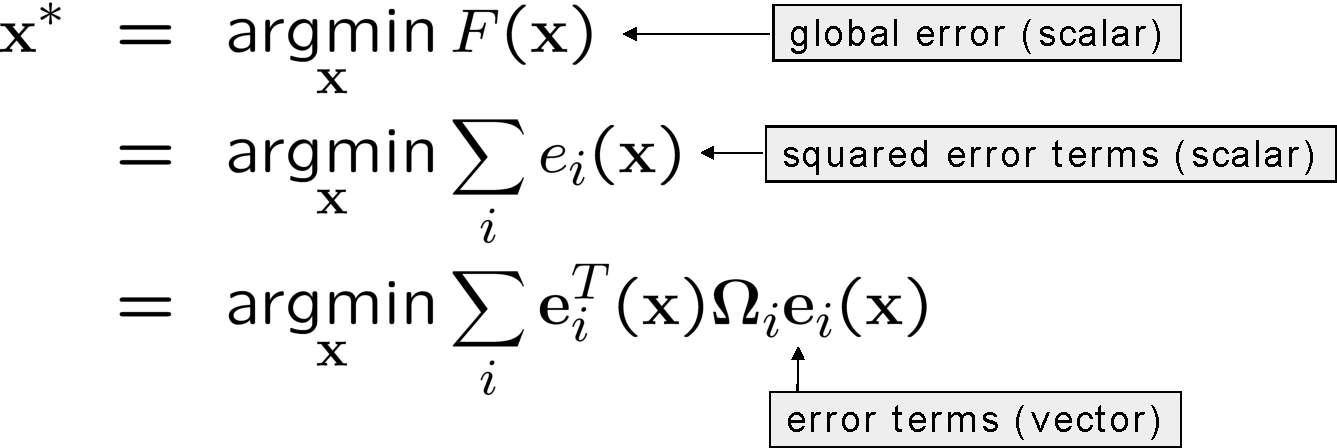
\includegraphics[width=0.7\textwidth]{images/find_minimum.pdf}
        \end{center}
    \end{itemize}

\end{frame}

\begin{frame}
    \frametitle{Objetivo: Encontrar el Mínimo}
    \note{Extraído de Curso de Cyrill Stachniss https://youtu.be/r2cyMQ5NB1o?si=WYODHSkWun3FL7jR}
    
    \begin{itemize}
        \item Encontrar el estado $\stateBold^{*}$ que minimiza el error dados todas las mediciones
        
        \begin{equation*}
            \stateBold^{*} = \argmin_{\stateBold} \sum_{i} \error_{i}\left( \stateBold \right)^{\top} \informationMatrix_{i} \error_{i}\left( \stateBold \right)
        \end{equation*}
        
        
        \item Una solución general es derivar la función de error global y encontrar sus nulos
        \item En general compleja y con solución no cerrada $\rightarrow$ Solución con Métodos numéricos
    \end{itemize}
    
\end{frame}


\begin{frame}
    \frametitle{Suposiciones}
    \note{Extraído de Curso de Cyrill Stachniss https://youtu.be/r2cyMQ5NB1o?si=WYODHSkWun3FL7jR}
    \begin{itemize}
        \item Hay una ``buena'' solución inicial disponible
        \item Las funciones de error son ``suaves'' en la vecindad del mínimo (con suerte global)
        \item Entonces, podemos resolver el problema con linearizaciones locales iterativas
    \end{itemize}

\end{frame}

\begin{frame}
    \frametitle{Resolvemos utilizando Linearizaciones locales iterativas}
    \note{Extraído de Curso de Cyrill Stachniss https://youtu.be/r2cyMQ5NB1o?si=WYODHSkWun3FL7jR}
    \begin{itemize}
        \item Linealizar los términos de error alrededor del solución actual/solución inicial
        \item Calcular la primera derivada de la función de error al cuadrado
        \item Setear en cero y resolver el sistema lineal
        \item Obtener el nuevo estado (que con suerte estará más cerca del mínimo)
        \item Iterar
    \end{itemize}
\end{frame}

\begin{frame}
    \frametitle{Linearizar la Función de Error}
    \note{Extraído de Curso de Cyrill Stachniss https://youtu.be/r2cyMQ5NB1o?si=WYODHSkWun3FL7jR}
    
    \begin{itemize}
        \item Podemos aproximar el error al rededor de una estimación inicial $\stateBold$ a través de una expansión de Taylor
    \end{itemize}
    
    \begin{equation*}
        \error_{i}(\stateBold + \vec{\Delta}\stateBold) \simeq  \underbrace{\error_{i}(\stateBold)}_{\error_{i}} + \jacobian_{i}\vec{\Delta}\stateBold \quad \text{con} \quad \jacobian_{i} = \dfrac{\partial\error_{i}(\stateBold)}{\partial\stateBold}
    \end{equation*}
    
\end{frame}

\begin{frame}
    \frametitle{Error Cuadrático}
    \note{Extraído de Curso de Cyrill Stachniss https://youtu.be/r2cyMQ5NB1o?si=WYODHSkWun3FL7jR}
    
    \begin{itemize}
        \item Con la linealización anterior, podemos fijar $\stateBold$ y llevar a cabo la minimización en los incrementos $\Delta\stateBold$
        \item Reemplazamos la expansión de Taylor en los términos de error al cuadrado:
        \only<1>{
            \begin{align*}
                e_{i}(\stateBold + \vec{\Delta}\stateBold) &= \dots
            \end{align*}
        }
        \only<2>{
            \begin{align*}
                e_{i}(\stateBold + \vec{\Delta}\stateBold) &= \error_{i}\left( \stateBold + \Delta \stateBold \right)^{\top} \informationMatrix_{i} \error_{i}\left( \stateBold  + \Delta \stateBold \right)
            \end{align*}
        }
        \only<3>{
            \begin{align*}
                e_{i}(\stateBold + \vec{\Delta}\stateBold) &= \error_{i}\left( \stateBold + \Delta \stateBold \right)^{\top} \informationMatrix_{i} \error_{i}\left( \stateBold  + \Delta \stateBold \right)\\
                &\simeq \left( \error_{i} + \jacobian_{i} \Delta \stateBold \right)^{\top} \informationMatrix_{i} \left( \error_{i} + \jacobian_{i} \Delta \stateBold \right)
            \end{align*}
        }
        \only<4>{
            \begin{align*}
                e_{i}(\stateBold + \vec{\Delta}\stateBold) &= \error_{i}\left( \stateBold + \Delta \stateBold \right)^{\top} \informationMatrix_{i} \error_{i}\left( \stateBold  + \Delta \stateBold \right)\\
                &\simeq \left( \error_{i} + \jacobian_{i} \Delta \stateBold \right)^{\top} \informationMatrix_{i} \left( \error_{i} + \jacobian_{i} \Delta \stateBold \right)\\
                &= \error_{i}^{\top} \informationMatrix_{i} \error_{i} + \error_{i}^{\top} \informationMatrix_{i} \jacobian_{i} \Delta \stateBold + \Delta \stateBold^{\top} \jacobian_{i}^{\top} \informationMatrix_{i} \error_{i} +  \Delta \stateBold^{\top} \jacobian_{i}^{\top} \informationMatrix_{i} \jacobian_{i} \Delta \stateBold
            \end{align*}
        }
    \end{itemize}
\end{frame}

\begin{frame}
    \frametitle{Error Cuadrático (cont.)}
    \note{Extraído de Curso de Cyrill Stachniss https://youtu.be/r2cyMQ5NB1o?si=WYODHSkWun3FL7jR}
    
    \begin{itemize}
        \item Todos los sumandos son escalares por lo que la transposición no tiene ningún efecto
        \item Agrupando términos similares obtenemos:
        \only<1>{
            \begin{align*}
                e_{i}(\stateBold + \vec{\Delta}\stateBold) &\simeq \error_{i}^{\top} \informationMatrix_{i} \error_{i} + \error_{i}^{\top} \informationMatrix_{i} \jacobian_{i} \Delta \stateBold + \Delta \stateBold^{\top} \jacobian_{i}^{\top} \informationMatrix_{i} \error_{i} +  \Delta \stateBold^{\top} \jacobian_{i}^{\top} \informationMatrix_{i} \jacobian_{i} \Delta \stateBold
            \end{align*}
        }
        \only<2>{
            \begin{align*}
                e_{i}(\stateBold + \vec{\Delta}\stateBold) &\simeq \error_{i}^{\top} \informationMatrix_{i} \error_{i} + \error_{i}^{\top} \informationMatrix_{i} \jacobian_{i} \Delta \stateBold + \Delta \stateBold^{\top} \jacobian_{i}^{\top} \informationMatrix_{i} \error_{i} +  \Delta \stateBold^{\top} \jacobian_{i}^{\top} \informationMatrix_{i} \jacobian_{i} \Delta \stateBold \\
                &= \underbrace{\error_{i}^{\top} \informationMatrix_{i} \error_{i}}_{c_{i}} + 2 \underbrace{\error_{i}^{\top} \informationMatrix_{i} \jacobian_{i}}_{\linearSystemb^{\top}_{i}} \Delta \stateBold + \Delta \stateBold^{\top} \underbrace{\jacobian_{i}^{\top} \informationMatrix_{i} \jacobian_{i}}_{\linearSystemH_{i}} \Delta \stateBold
            \end{align*}
        }
        \only<3>{
            \begin{align*}
                e_{i}(\stateBold + \vec{\Delta}\stateBold) &\simeq \error_{i}^{\top} \informationMatrix_{i} \error_{i} + \error_{i}^{\top} \informationMatrix_{i} \jacobian_{i} \Delta \stateBold + \Delta \stateBold^{\top} \jacobian_{i}^{\top} \informationMatrix_{i} \error_{i} +  \Delta \stateBold^{\top} \jacobian_{i}^{\top} \informationMatrix_{i} \jacobian_{i} \Delta \stateBold \\
                &= \underbrace{\error_{i}^{\top} \informationMatrix_{i} \error_{i}}_{c_{i}} + 2 \underbrace{\error_{i}^{\top} \informationMatrix_{i} \jacobian_{i}}_{\linearSystemb^{\top}_{i}} \Delta \stateBold + \Delta \stateBold^{\top} \underbrace{\jacobian_{i}^{\top} \informationMatrix_{i} \jacobian_{i}}_{\linearSystemH_{i}} \Delta \stateBold \\
                &= c_{i} + 2 \linearSystemb^{\top}_{i} \Delta \stateBold + \Delta \stateBold^{\top} \linearSystemH_{i} \Delta \stateBold
            \end{align*}
        }
    \end{itemize}
    
    
\end{frame}

\begin{frame}
    \frametitle{Error Global}
    \note{Extraído de Curso de Cyrill Stachniss https://youtu.be/r2cyMQ5NB1o?si=WYODHSkWun3FL7jR}
    
    \begin{itemize}
        \item El error global es la suma de términos de errores cuadrados correspondientes a las medidas individuales
        \item Forma una nueva expresión, que se aproxima al error global en la vecindad de la solución actual $\stateBold$
    \end{itemize}
    
    \begin{align*}
        F\left(\stateBold + \Delta \stateBold \right) &= \sum_{i} e_{i}(\stateBold + \vec{\Delta}\stateBold)\\
        F\left(\stateBold + \Delta \stateBold \right) &\simeq \sum_{i} \left( c_{i} + 2 \linearSystemb^{\top}_{i} \Delta \stateBold + \Delta \stateBold^{\top} \linearSystemH_{i} \Delta \stateBold \right) \\
        &= \sum_{i} c_{i} + 2 \left( \sum_{i} \linearSystemb^{\top}_{i} \right) \Delta \stateBold + \Delta \stateBold^{\top} \left( \sum_{i} \linearSystemH_{i} \right) \Delta \stateBold
    \end{align*}
    
    
\end{frame}

\begin{frame}
    \frametitle{Error Global (cont.)}
    \note{Extraído de Curso de Cyrill Stachniss https://youtu.be/r2cyMQ5NB1o?si=WYODHSkWun3FL7jR}
    
    \begin{align*}
        F\left(\stateBold + \Delta \stateBold \right) &\simeq \sum_{i} \left( c_{i} + 2 \linearSystemb^{\top}_{i} \Delta \stateBold + \Delta \stateBold^{\top} \linearSystemH_{i} \Delta \stateBold \right) \\
        &= \underbrace{\sum_{i} c_{i}}_{c} + 2 \underbrace{\left( \sum_{i} \linearSystemb^{\top}_{i} \right)}_{\linearSystemb^{\top}} \Delta \stateBold + \Delta \stateBold^{\top} \underbrace{\left( \sum_{i} \linearSystemH_{i} \right)}_{\linearSystemH} \Delta \stateBold \\
        &= c + 2 \linearSystemb^{\top} \Delta \stateBold + \Delta \stateBold^{\top} \linearSystemH \Delta \stateBold
    \end{align*}
    
    con
    
    \begin{align*}
        \linearSystemb^{\top} &= \sum_{i} \error_{i}^{\top} \informationMatrix_{i} \jacobian_{i} \\ 
        \linearSystemH &= \sum_{i}  \jacobian_{i}^{\top} \informationMatrix_{i} \jacobian_{i}
    \end{align*}
    
    
\end{frame}

\begin{frame}
    \frametitle{Forma Cuadrática}
    \note{Extraído de Curso de Cyrill Stachniss https://youtu.be/r2cyMQ5NB1o?si=WYODHSkWun3FL7jR}
    
    \begin{itemize}
        \item<1-> Podemos escribir los términos de error global como una forma cuadrática en $\Delta \stateBold$
        
        \begin{equation*}
            F\left(\stateBold + \Delta \stateBold \right) = c + 2 \linearSystemb^{\top} \Delta \stateBold + \Delta \stateBold^{\top} \linearSystemH \Delta \stateBold
        \end{equation*}
        
        \item<1> \alert{¿Cómo calcular el mínimo de una forma cuadrática?}
        \item<2-> Calcular la derivada de  $F\left(\stateBold + \Delta \stateBold \right)$ con respecto a $\Delta \stateBold$ (dado $\stateBold$)
        \item<2-> Derivamos e igualamos a 0
        \item<2-> resolvemos
    \end{itemize}

\end{frame}

\begin{frame}
    \frametitle{Derivando la forma cuadrática}
    \note{Extraído de Curso de Cyrill Stachniss https://youtu.be/r2cyMQ5NB1o?si=WYODHSkWun3FL7jR}
    
    \begin{itemize}
        \item Dada la forma cuadrática
        \begin{equation*}
            f(\stateBold) = \stateBold^{\top} \linearSystemH \stateBold + \linearSystemb^{\top} \stateBold
        \end{equation*}
        \item La primera derivada es
        \begin{equation*}
            \dfrac{\partial f}{\partial \stateBold} = \left( \linearSystemH + \linearSystemH^{\top} \right) \stateBold + \linearSystemb
        \end{equation*}
    \end{itemize}
    
    Ver: The Matrix Cookbook, sección 2.4.2
   
\end{frame}

\begin{frame}
    \frametitle{Forma Cuadrática}
    \note{Extraído de Curso de Cyrill Stachniss https://youtu.be/r2cyMQ5NB1o?si=WYODHSkWun3FL7jR}
    
    \begin{itemize}
        \item Podemos escribir los términos de error global de forma cuadrática en $\Delta \stateBold$
        \begin{equation*}
            F\left(\stateBold + \Delta \stateBold \right) = c + 2 \linearSystemb^{\top} \Delta \stateBold + \Delta \stateBold^{\top} \linearSystemH \Delta \stateBold
        \end{equation*}
        \item La derivada de $F\left(\stateBold + \Delta \stateBold \right)$
        \begin{equation*}
            \dfrac{\partial F\left(\stateBold + \Delta \stateBold \right)}{\partial \Delta \stateBold} \simeq 2 \linearSystemb + 2 \linearSystemH \Delta \stateBold
        \end{equation*}
    \end{itemize}
    
\end{frame}

\begin{frame}
    \frametitle{Minimizando la forma cuadrática}
    \note{Extraído de Curso de Cyrill Stachniss https://youtu.be/r2cyMQ5NB1o?si=WYODHSkWun3FL7jR}
    
    \begin{itemize}
        \item Derivada de $F\left(\stateBold + \Delta \stateBold \right)$
        \begin{equation*}
            \dfrac{\partial F\left(\stateBold + \Delta \stateBold \right)}{\partial \Delta \stateBold} \simeq 2 \linearSystemb + 2 \linearSystemH \Delta \stateBold
        \end{equation*}
        \item Igualando a 0
        \begin{equation*}
            0 = 2 \linearSystemb + 2 \linearSystemH \Delta \stateBold
        \end{equation*}
        \item Lo que lleva al sistema lineal
        \begin{equation*}
            \linearSystemH \Delta \stateBold = -\linearSystemb 
        \end{equation*}
        \item La solución para el incremento $\Delta \stateBold^{*}$ es
        \begin{equation*}
             \Delta \stateBold^{*} = - \inverse{\linearSystemH} \linearSystemb 
        \end{equation*}
    \end{itemize}
    
\end{frame}

\begin{frame}
    \frametitle{Solución con Gauss-Newton}
    \note{Extraído de Curso de Cyrill Stachniss https://youtu.be/r2cyMQ5NB1o?si=WYODHSkWun3FL7jR}
    
    Iterar los siguientes pasos:
    \begin{itemize}
        \item Lineanizar cerca de $\stateBold$ y computar para cada medición
        \begin{equation*}
            \error_{i}(\stateBold + \vec{\Delta}\stateBold) \simeq  \error_{i}(\stateBold) + \jacobian_{i}\vec{\Delta}\stateBold
        \end{equation*}
        \item Computar los términos del sistema lineal
        \begin{equation*}
            \linearSystemb^{\top} = \sum_{i} \error_{i}^{\top} \informationMatrix_{i} \jacobian_{i} \quad \quad \linearSystemH = \sum_{i} \jacobian_{i}^{\top} \informationMatrix_{i} \jacobian_{i}
        \end{equation*}
    \item Resolver el sistema lineal
    \begin{equation*}
        \Delta \stateBold^{*} = - \inverse{\linearSystemH} \linearSystemb 
    \end{equation*}
    \item Actualizar el estado
    \begin{equation*}
        \stateBold \leftarrow \stateBold + \Delta \stateBold^{*}
    \end{equation*} 
    \end{itemize}
    
\end{frame}

\begin{frame}
    \frametitle{Ejemplo: Calibración de Odometría}
    \note{Extraído de Curso de Cyrill Stachniss https://youtu.be/r2cyMQ5NB1o?si=WYODHSkWun3FL7jR}
    
    \begin{itemize}
        \item Mediciones de Odometría $\controlCommand_{i}$
        \item Eliminar el error sistemático a través de la calibración
        \item Suposición: disponemos del ground-truth de odometría $\controlCommand_{i}^{*}$
        \item Ground-truth dado por sistemas: Motion Capture (Vicon), Scan-Matching o SLAM
    \end{itemize}
    
\end{frame}

\begin{frame}
    \frametitle{Ejemplo: Calibración de Odometría}
    \note{Extraído de Curso de Cyrill Stachniss https://youtu.be/r2cyMQ5NB1o?si=WYODHSkWun3FL7jR}
    
    \begin{itemize}
        \item Hay una función que $f_{i}(\stateBold)$ que dado algunos parámetros de bias $\stateBold$, devuelve una odometría corregida (\emph{unbiased}) para la lectura ruidosa $\controlCommand_{i}^{\prime}$ 
        \begin{equation*}
            \controlCommand_{i}^{\prime} = f_{i}(\stateBold) =
            \begin{bmatrix}
                x_{11} & x_{12} & x_{13} \\
                x_{21} & x_{22} & x_{23} \\
                x_{31} & x_{32} & x_{33}
            \end{bmatrix}
            \controlCommand_{i}
        \end{equation*}
    \item Para obtener la función de corrección $f(\stateBold)$, necesitamos encontrar los parámetros $\stateBold$
    \end{itemize}
    
\end{frame}

\begin{frame}
    \frametitle{Calibración de Odoemtría (cont.)}
    \note{Extraído de Curso de Cyrill Stachniss https://youtu.be/r2cyMQ5NB1o?si=WYODHSkWun3FL7jR}
    \begin{itemize}

        \item El vector estado es 
        \begin{equation*}
            \stateBold =
            \begin{bmatrix}
                x_{11} & x_{12} & x_{13} & x_{21} & x_{22} & x_{23} & x_{31} & x_{32} & x_{33}
            \end{bmatrix}
        \end{equation*}
        \item La función error es
        \begin{equation*}
            \error_{i}(\stateBold) = \controlCommand_{i}^{*} - 
            \begin{bmatrix}
                x_{11} & x_{12} & x_{13} \\
                x_{21} & x_{22} & x_{23} \\
                x_{31} & x_{32} & x_{33}
            \end{bmatrix}
            \controlCommand_{i}
        \end{equation*}
        \item Su derivada es
        
    %    \begin{equation*}
    %        \jacobian_{i} = \dfrac{\partial \error_{i}(\stateBold)}{\partial \stateBold} = -
    %        \begin{bmatrix}
    %            u_{i,x} & u_{i,y} & u_{i,\theta} & 0 & 0 & 0 & 0 & 0 & 0 \\
    %            0 & 0 & 0 & u_{i,x} & u_{i,y} & u_{i,\theta} & 0 & 0 & 0 \\
    %            0 & 0 & 0 & 0 & 0 & 0 & u_{i,x} & u_{i,y} & u_{i,\theta}
    %        \end{bmatrix}
    %    \end{equation*}
    
        \begin{center}
            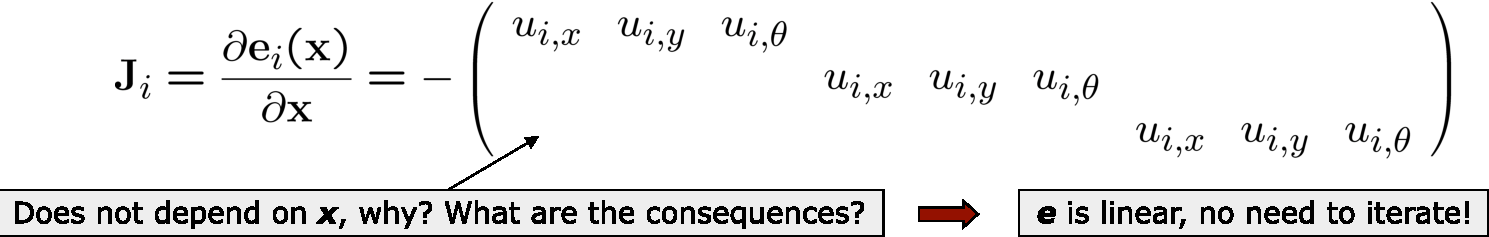
\includegraphics[width=0.8\columnwidth]{images/odometry_calibration_jacobian.pdf}
        \end{center}
        
        Que la primera derivada (Jacobiano) no dependa de $\stateBold$, es lo menos común, ya que significa que la función $\error$ es lineal!
        
        En este caso solo vamos a tener que hacer una sola iteración.

    \end{itemize}

    
\end{frame}

\begin{frame}
    \frametitle{Preguntas}
    \note{Extraído de Curso de Cyrill Stachniss https://youtu.be/r2cyMQ5NB1o?si=WYODHSkWun3FL7jR}
    
    \begin{itemize}
        \item<1-> ¿Cómo lucen los parámetros si la odometría es perfecta?
        \begin{itemize}
            \item<2-> La matriz debería ser la identidad. Entonces el error es 0, y por lo tanto, encontramos el mínimo.
        \end{itemize}
        \item<3-> ¿Cuantas mediciones son necesarias para encontrar la solución al problema de calibración?
        \begin{itemize}
            \item<4-> Tenemos que ver cuantas variables desconocidas tenemos y cuanta información nos provee cada observación. Tenemos 9 variables desconocidas. Cada observación nos da información de 3 variables (nos da 3 ecuaciones). Por lo tanto, vamos a necesitar al menos 3 observaciones.
        \end{itemize}
        \item<5-> $\linearSystemH$ es simétrica. ¿Por qué?
        \begin{itemize}
            \item<6-> La forma en que $\linearSystemH$ es simétrica porque  $\linearSystemH = \jacobian^{\top}\Omega\jacobian$. $\Omega$ es simétrica definida postiva y $\jacobian$ tambien, y por lo tanto el producto también.
        \end{itemize}
        \item<7-> ¿Cómo afecta la estructura de la función de medición a la estructura de $\linearSystemH$?
        \begin{itemize}
            \item<8-> $\linearSystemH$ es esparsa porque los jacobianos son esparsos. Los jacobianos son esparsos porque codifican cuanta información nos da una medición sobre todas las variables de estado. Por lo tanto, si nuestras mediciones solo relacionan algunas variables (como es el caso de SLAM), entonces la $\linearSystemH$ será esparsa.
        \end{itemize}
    \end{itemize}

\end{frame}

\begin{frame}
    \frametitle{¿Cómo Resolver de manera eficiente un Sistema Lineal?}
    \note{Extraído de Curso de Cyrill Stachniss https://youtu.be/r2cyMQ5NB1o?si=WYODHSkWun3FL7jR}
    \begin{itemize}
        \item Sistema Lineal $\linearSystemH \Delta \stateBold = -\linearSystemb$
        \item Podemos resolverlo utilizando inversión de matrices (en teoría)
        \item En la práctica:
        \begin{itemize}
            \item Factorización de Cholesky
            \item Descomposición QR
            \item Métodos iterativos como el método del Gradiente Conjugado (para sistemas grandes)
        \end{itemize}
        
    \end{itemize}
    
\end{frame}

\begin{frame}
    \frametitle{Descomposición de Cholesky para Resolver un Sistema Lineal}
    \note{Extraído de Curso de Cyrill Stachniss https://youtu.be/r2cyMQ5NB1o?si=WYODHSkWun3FL7jR}
    
    \begin{itemize}
        \item Sea la matriz $\vec{A}$ simétrica positiva definida
        \item El sistema a resolver es $\vec{A} \vec{x} = \vec{b}$
        \item Cholesky lleva a $\vec{A} = \vec{L} \vec{L}^{\top}$ con $\vec{L}$ matriz triangular inferior
        \item<2> Resolvemos primero
        \begin{equation*}
            \vec{L} \vec{y} = \vec{b}
        \end{equation*}
        \item<2> y luego,
        \begin{equation*}
            \vec{L}^{\top} \vec{x} = \vec{y}
        \end{equation*}
    
    \end{itemize}
    
\end{frame}

\begin{frame}
    \frametitle{Resumen de Gauss-Newton}
    \note{Extraído de Curso de Cyrill Stachniss https://youtu.be/r2cyMQ5NB1o?si=WYODHSkWun3FL7jR}
    
    Método para minimizar un error al cuadrado:
    \begin{itemize} 
        \item Comenzar con una solución inicial (\emph{initial guess})
        \item Linealizar las funciones de error individuales
        \item Esto lleva a una forma cuadrática
        \item Se obtiene un sistema lineal derivando e igualando a 0
        \item Resolver el sistema lineal conduce a una actualización del estado
        \item Iterar
    \end{itemize}
    
\end{frame}

\begin{frame}
    \frametitle{Least Squares vs. Probabilistic State Estimation}
    \note{Extraído de Curso de Cyrill Stachniss https://youtu.be/r2cyMQ5NB1o?si=WYODHSkWun3FL7jR}
    
    \begin{itemize}
        \item Hasta ahora, minimizamos una función de error
        \item ¿Cómo se relaciones esto con la estimación de estado en el sentido probabilístico?
    \end{itemize}
    
\end{frame}

\begin{frame}
    \frametitle{Comencemos con Estimación de estado}
    \note{Extraído de Curso de Cyrill Stachniss https://youtu.be/r2cyMQ5NB1o?si=WYODHSkWun3FL7jR}
    
    \begin{itemize}
        \item Regla de Bayes, suposiciones de independencia y Markov nos permiten reescribir
        \begin{equation*}
            p\left( \state_{0:t} | \observation_{1:t}, \controlCommand_{1:t} \right) = \eta p\left( \state_{0} \right) \prod_{t} \left[ p\left( \state_{t} | \state_{t-1}, \controlCommand_{t} \right) p\left( \observation_{t} | \state_{t} \right) \right]
        \end{equation*}
    \end{itemize}
    
    \note{p(x0) es un prior. Observar que en x0 no tenemos observaciones ni comandos de control}
    
\end{frame}

\begin{frame}
    \frametitle{Log Likelihood}
    \note{Extraído de Curso de Cyrill Stachniss https://youtu.be/r2cyMQ5NB1o?si=WYODHSkWun3FL7jR}
    
    \begin{itemize}
        \item Reescribiendo como el log likelihood, lleva a
        \begin{equation*}
            \log p\left( \state_{0:t} | \observation_{1:t}, \controlCommand_{1:t} \right) = \text{const.}  \log p\left( \state_{0} \right) + \sum_{t} \left[ \log p\left( \state_{t} | \state_{t-1}, \controlCommand_{t} \right) + \log p\left( \observation_{t} | \state_{t} \right) \right]
        \end{equation*}
    \end{itemize}
    
\end{frame}

\begin{frame}
    \frametitle{Suposición Gaussiana}
    \note{Extraído de Curso de Cyrill Stachniss https://youtu.be/r2cyMQ5NB1o?si=WYODHSkWun3FL7jR}
    
    \begin{itemize}
        \item Suponiendo distribución Gaussiana
        \begin{equation*}
            \log p\left( \state_{0:t} | \observation_{1:t}, \controlCommand_{1:t} \right) = \text{const.}  \log \underbrace{p\left( \state_{0} \right)}_{\mathcal{N}} + \sum_{t} \left[ \log \underbrace{p\left( \state_{t} | \state_{t-1}, \controlCommand_{t} \right)}_{\mathcal{N}} + \log \underbrace{p\left( \observation_{t} | \state_{t} \right)}_{\mathcal{N}} \right]
        \end{equation*}
    \end{itemize}
    
\end{frame}

\begin{frame}
    \frametitle{Log de una Gaussiana}
    \note{Extraído de Curso de Cyrill Stachniss https://youtu.be/r2cyMQ5NB1o?si=WYODHSkWun3FL7jR}

    
    \begin{itemize}
        \item La función de distribución de la distribución normal está definida como
        \begin{equation*}
            p(x)=\det(2\pi\covariance)^{\frac{1}{2}} \exp\left(-\dfrac{1}{2} (x - \mu )^{\top} \inverse{\covariance} (x - \mu )  \right)
        \end{equation*}
        
        \item Log likelihood de una Gaussiana
        \begin{equation*}
            \log \mathcal{N}(x, \mu, \Sigma) =  \text{const.} - \dfrac{1}{2} (x - \mu)^{\top} \inverse{\Sigma} (x - \mu)
        \end{equation*}
    \end{itemize}
    
\end{frame}

\begin{frame}
    \frametitle{Función de Error como Exponente}
    \note{Extraído de Curso de Cyrill Stachniss https://youtu.be/r2cyMQ5NB1o?si=WYODHSkWun3FL7jR}
    
    \begin{itemize}
        \item Log likelihood de una Gaussiana
        \begin{equation*}
            \log \mathcal{N}(x, \mu, \Sigma) =  \text{const.} - \dfrac{1}{2} \underbrace{\underbrace{(x - \mu)^{\top}}_{\error^{\top}(x)} \underbrace{\inverse{\Sigma}}_{\informationMatrix} \underbrace{(x - \mu)}_{\error(x)}}_{e(x)}
        \end{equation*}
        \item está a una constante de equivalencia de las funciones de error usadas antes
    \end{itemize}
    
\end{frame}

\begin{frame}
    \frametitle{Log Likelihood con Términos de Error}
    \note{Extraído de Curso de Cyrill Stachniss https://youtu.be/r2cyMQ5NB1o?si=WYODHSkWun3FL7jR}
    
    \begin{itemize}
        \item Suponiendo distribución Gaussiana
        \begin{equation*}
            \log p\left( \state_{0:t} | \observation_{1:t}, \controlCommand_{1:t} \right) = \text{const.} - \dfrac{1}{2} e_{p}(\state) -  \dfrac{1}{2} \sum_{t} \left[ e_{\controlCommand_{t}}(\state) + e_{\observation_{t}}(\state)\right]
        \end{equation*}
    \end{itemize}
    
\end{frame}

\begin{frame}
    \frametitle{Maximizing el Log Likelihood}
    \note{Extraído de Curso de Cyrill Stachniss https://youtu.be/r2cyMQ5NB1o?si=WYODHSkWun3FL7jR}
    
    \begin{itemize}
        \item Suponiendo distribución Gaussiana
        \begin{equation*}
            \log p\left( \state_{0:t} | \observation_{1:t}, \controlCommand_{1:t} \right) = \text{const.} - \dfrac{1}{2} e_{p}(\state) -  \dfrac{1}{2} \sum_{t} \left[ e_{\controlCommand_{t}}(\state) + e_{\observation_{t}}(\state)\right]
        \end{equation*}
        \item Maximizando el log likelihood lleva a 
        \begin{equation*}
            \argmax \log p\left( \state_{0:t} | \observation_{1:t}, \controlCommand_{1:t} \right) = \argmin e_{p}(\state) + \sum_{t} \left[ e_{\controlCommand_{t}}(\state) + e_{\observation_{t}}(\state)\right]
        \end{equation*}
    \end{itemize}
    
    
\end{frame}

\begin{frame}
    \frametitle{Minimizar el error cuadrático es equivalente a Maximizar el Log Likelihood de Distribuciones Gaussianas Independientes}
    \note{Extraído de Curso de Cyrill Stachniss https://youtu.be/r2cyMQ5NB1o?si=WYODHSkWun3FL7jR}
    \begin{itemize}
        \item Con términos de error individuales para los controles, mediciones y un prior:
        \begin{equation*}
            \argmax \log p\left( \state_{0:t} | \observation_{1:t}, \controlCommand_{1:t} \right) = \argmin e_{p}(\state) + \sum_{t} \left[ e_{\controlCommand_{t}}(\state) + e_{\observation_{t}}(\state)\right]
        \end{equation*}
    \end{itemize}
    
\end{frame}

\begin{frame}
    \frametitle{Resumen}
    \note{Extraído de Curso de Cyrill Stachniss https://youtu.be/r2cyMQ5NB1o?si=WYODHSkWun3FL7jR}
    
    \begin{itemize}
        \item Técnica para minimizar funciones de error cuadráticas
        \item Gauss-Newton es un enfoque iterativo para problemas no lineales
        \item Utiliza linearización (¡aproximación!)
        \item Equivalente a maximizar el log likelihood de Gaussianas independientes
        \item Método popular en muchas disciplinas.
    \end{itemize}

    
\end{frame}

\begin{frame}
    \frametitle{Bibliografía de Gauss-Newton}
    \note{Extraído de Curso de Cyrill Stachniss https://youtu.be/r2cyMQ5NB1o?si=WYODHSkWun3FL7jR}
    \begin{itemize}
        \item Capítulo 11.4 de \cite{thrun2005probabilistic}
    \end{itemize}
\end{frame}